%%
% The BIThesis Template for Bachelor Graduation Thesis
%
% 北京理工大学毕业设计(论文) —— 使用 XeLaTeX 编译
%
% Copyright 2020 Spencer Woo
%
% This work may be distributed and/or modified under the
% conditions of the LaTeX Project Public License, either version 1.3
% of this license or (at your option) any later version.
% The latest version of this license is in
%   http://www.latex-project.org/lppl.txt
% and version 1.3 or later is part of all distributions of LaTeX
% version 2005/12/01 or later.
%
% This work has the LPPL maintenance status `maintained'.
%
% The Current Maintainer of this work is Spencer Woo.
%
% Compile with: xelatex -> biber -> xelatex -> xelatex

% 章节支持、单面打印:ctexbook
\documentclass[UTF8,AutoFakeBold,AutoFakeSlant,zihao=-4,oneside,openany]{ctexbook}
\usepackage[a4paper,left=3cm,right=2.6cm,top=3.5cm,bottom=2.9cm]{geometry}
% 目前 29mm 最接近 Word 排版
\usepackage{xeCJK}
\usepackage{titletoc}
\usepackage{titlesec}
\usepackage{fontspec}
\usepackage{setspace}
\usepackage{graphicx}
\usepackage{fancyhdr}
\usepackage{pdfpages}
\usepackage{setspace}
\usepackage{booktabs}
\usepackage{multirow}
\usepackage{caption}
\usepackage{tikz}
\usepackage{etoolbox}
\usepackage{hyperref}
\usepackage{xcolor}
\usepackage{caption}
\usepackage{array}
\usepackage{amsmath}
\usepackage{amssymb}
\usepackage{pdfpages}
\usepackage[ruled,vlined]{algorithm2e}
\usepackage{listings}
\usepackage{float}
\usepackage{iitem}
% \usepackage{minted}
% 设置参考文献编译后端为 biber,引用格式为 GB/T7714-2015 格式
% 参考文献使用宏包见 https://github.com/hushidong/biblatex-gb7714-2015
\lstdefinelanguage
   [x64]{Assembler}     % add a "x64" dialect of Assembler
   [x86masm]{Assembler} % based on the "x86masm" dialect
   % with these extra keywords:
   {morekeywords={CDQE,CQO,CMPSQ,CMPXCHG16B,JRCXZ,LODSQ,MOVSXD, %
                  POPFQ,PUSHFQ,SCASQ,STOSQ,IRETQ,RDTSCP,SWAPGS, %
                  rax,rdx,rcx,rbx,rsi,rdi,rsp,rbp, %
                  r8,r8d,r8w,r8b,r9,r9d,r9w,r9b, %
                  r10,r10d,r10w,r10b,r11,r11d,r11w,r11b, %
                  r12,r12d,r12w,r12b,r13,r13d,r13w,r13b, %
                  r14,r14d,r14w,r14b,r15,r15d,r15w,r15b}} % etc.

\lstset{language=[x64]Assembler}

\lstset{
    numbers=left, 
    numberstyle= \tiny, 
    keywordstyle= \color{ blue!70},
    commentstyle= \color{red!50!green!50!blue!50}, 
    frame=shadowbox, % 阴影效果
    rulesepcolor= \color{ red!20!green!20!blue!20} ,
    escapeinside=``, % 英文分号中可写入中文
    % xleftmargin=2em,xrightmargin=2em, aboveskip=1em,
    % framexleftmargin=2em
} 

\usepackage[
  backend=biber,
  style=gb7714-2015,
  gbalign=gb7714-2015,
  gbnamefmt=lowercase,
  gbpub=false,
  doi=false,
  url=false,
  eprint=false,
  isbn=false,
]{biblatex}

% 参考文献引用文件位于 misc/ref.bib
\addbibresource{misc/ref.bib}

% 西文字体默认为 Times New Roman
\setromanfont{Times New Roman}
% 论文题目字体为华文细黑
\setCJKfamilyfont{xihei}{[STXIHEI.TTF]} % 若希望使用本机字体,也可以用 {STXihei} 来调用
\newcommand{\xihei}{\CJKfamily{xihei}}

% 在这里填写你的论文中英文题目
\newcommand{\thesisTitle}{基于MASM的汇编程序设计}
\newcommand{\thesisTitleEN}{Assembly programming based on MASM}

% 在这里填写你的相关信息
\newcommand{\deptName}{计算机学院}
\newcommand{\majorName}{计算机科学与技术}
\newcommand{\yourName}{唐小娟}
\newcommand{\yourStudentID}{1120180207}
\newcommand{\mentorName}{李元章}
% 如果你的毕设为校外毕设,请将下面这一行语句解除注释(删除第一个百分号字符)并在第二组花括号中填写你的校外毕设导师名字
% \newcommand{\externalMentorName}{左偏树}

% 主题页面格式:BIThesis
\fancypagestyle{BIThesis}{
  % 页眉高度
  \setlength{\headheight}{20pt}
  % 页码高度(不完美,比规定稍微靠下 2mm)
  \setlength{\footskip}{14pt}

  \fancyhf{}
  % 定义页眉、页码
  \fancyhead[C]{\zihao{4}\ziju{0.08}\songti{北京理工大学本科生毕业设计(论文)}}
  \fancyfoot[C]{\songti\zihao{5} \thepage}
  % 页眉分割线稍微粗一些
  \renewcommand{\headrulewidth}{0.6pt}
}

% 设置章节格式
% 一级标题:黑体,三号,加粗;间距:段前 0.5 行,段后 1 行;
% \titleclass{\chapter}{straight}
% \titleformat{\chapter}[display]
%   {\normalfont\huge\bfseries}
%   {\chaptertitlename\ \thechapter}
%   {20pt}
%   {\Huge}
% \titlespacing*{\chapter} {0pt}{50pt}{40pt}

\ctexset{chapter={
    name = {第,章},
    number = {\arabic{chapter}},
    format = {\heiti \bfseries \centering \zihao{3}},
    aftername = \hspace{9bp},
    pagestyle = BIThesis,
    beforeskip = 8bp,
    afterskip = 32bp,
    fixskip = true,
  }
}

% 二级标题:黑体,四号,加粗;间距:段前 0.5 行,段后 0 行;
\ctexset{section={
    number = {\thechapter.\hspace{4bp}\arabic{section}},
    format = {\heiti \raggedright \bfseries \zihao{4}},
    aftername = \hspace{8bp},
    beforeskip = 20bp plus 1ex minus .2ex,
    afterskip = 18bp plus .2ex,
    fixskip = true,
  }
}

% 三级标题:黑体、小四、加粗;间距:段前 0.5 行,段后 0 行;
\ctexset{subsection={
    number = {\thechapter.\hspace{3bp}\arabic{section}.\hspace{3bp}\arabic{subsection}},
    format = {\heiti \bfseries \raggedright \zihao{-4}},
    aftername = \hspace{7bp},
    beforeskip = 17bp plus 1ex minus .2ex,
    afterskip = 14bp plus .2ex,
    fixskip = true,
  }
}

% 设置目录样式
% 添加 PDF 链接
\addtocontents{toc}{\protect\hypersetup{hidelinks}}

% 解决「目录」二字的格式问题
\renewcommand{\contentsname}{
  \fontsize{16pt}{\baselineskip}
  \normalfont\heiti{目~~~~录}
  \vspace{-8pt}
}
% 定义目录样式
\titlecontents{chapter}[0pt]{\songti \zihao{-4}}
{\thecontentslabel\hspace{\ccwd}}{}
{\hspace{.5em}\titlerule*{.}\contentspage}
\titlecontents{section}[1\ccwd]{\songti \zihao{-4}}
{\thecontentslabel\hspace{\ccwd}}{}
{\hspace{.5em}\titlerule*{.}\contentspage}
\titlecontents{subsection}[2\ccwd]{\songti \zihao{-4}}
{\thecontentslabel\hspace{\ccwd}}{}
{\hspace{.5em}\titlerule*{.}\contentspage}

% 前置页面(原创性声明、中英文摘要、目录等)
\renewcommand{\frontmatter}{
  \pagenumbering{Roman}
  \pagestyle{BIThesis}
}

% 正文页面
\renewcommand{\mainmatter}{
  \pagenumbering{arabic}
  \pagestyle{BIThesis}
}

% 设置 caption 与 figure 之间的距离
\setlength{\abovecaptionskip}{11pt}
\setlength{\belowcaptionskip}{9pt}

% 设置图片的 caption 格式
\renewcommand{\thefigure}{\thechapter-\arabic{figure}}
\captionsetup[figure]{font=small,labelsep=space}

% 设置表格的 caption 格式和 caption 与 table 之间的垂直距离
\renewcommand{\thetable}{\thechapter-\arabic{table}}
\captionsetup[table]{font=small,labelsep=space,skip=2pt}

% 调整底层 TeX 排版引擎参数以保证所有段落能够很好地以两端对齐的方式呈现
\tolerance=1
\emergencystretch=\maxdimen
\hyphenpenalty=10000
\hbadness=10000

% 设置数学公式编号格式
\renewcommand{\theequation}{\arabic{chapter}-\arabic{equation}}

\newcommand{\unnumchapter}[1]{
  \chapter*{\vskip 10bp\textmd{#1} \vskip -6bp}
  \addcontentsline{toc}{chapter}{#1}
  \stepcounter{chapter}
}

% 文档开始
\begin{document}

% 标题页面:如无特殊需要,本部分无需改动
%%
% The BIThesis Template for Bachelor Graduation Thesis
%
% 北京理工大学毕业设计(论文)封面页 —— 使用 XeLaTeX 编译
%
% Copyright 2020 Spencer Woo
%
% This work may be distributed and/or modified under the
% conditions of the LaTeX Project Public License, either version 1.3
% of this license or (at your option) any later version.
% The latest version of this license is in
%   http://www.latex-project.org/lppl.txt
% and version 1.3 or later is part of all distributions of LaTeX
% version 2005/12/01 or later.
%
% This work has the LPPL maintenance status `maintained'.
%
% The Current Maintainer of this work is Spencer Woo.
%
% 封面
%
% 如无特殊需要,本页面无需更改

% Underline new command for student information
% Usage: \dunderline[<offset>]{<line_thickness>}
\newcommand\dunderline[3][-1pt]{{%
  \setbox0=\hbox{#3}
  \ooalign{\copy0\cr\rule[\dimexpr#1-#2\relax]{\wd0}{#2}}}}

% Cover Page
\begin{titlepage}
  \makeatletter
  \@ifundefined{externalMentorName}{
    % 校内毕设封面顶部间距
    \vspace*{19mm}
  }{
    % 校外毕设封面顶部间距
    \vspace*{13mm}
  }
  \centering

  
\includegraphics[width=9.87cm]{images/header.png}

  \vspace*{-3mm}

  \zihao{-0}\textbf{\ziju{0.12}\songti{本科生毕业设计(论文)}}

  \vspace{16mm}

  \zihao{2}\textbf{\xihei\thesisTitle}

  \vspace{3mm}

  \begin{spacing}{1.2}
    \zihao{3}\selectfont{\textbf{\thesisTitleEN}}
  \end{spacing}

  \vspace{15mm}

  \flushleft

  \makeatletter
  \@ifundefined{externalMentorName}{
    % 生成校内毕设封面字段
    \makeatother
    \begin{spacing}{1.8}
      \hspace{27mm}\songti\zihao{3}\selectfont{学\hspace{11mm}院:\dunderline[-10pt]{1pt}{\makebox[78mm][c]{\deptName}}}

      \hspace{27mm}\songti\zihao{3}\selectfont{专\hspace{11mm}业:\dunderline[-10pt]{1pt}{\makebox[78mm][c]{\majorName}}}

      \hspace{27mm}\songti\zihao{3}\selectfont{学生姓名:\dunderline[-10pt]{1pt}{\makebox[78mm][c]{\yourName}}}

      \hspace{27mm}\songti\zihao{3}\selectfont{学\hspace{11mm}号:\dunderline[-10pt]{1pt}{\makebox[78mm][c]{\yourStudentID}}}

      \hspace{27mm}\songti\zihao{3}\selectfont{指导教师:\dunderline[-10pt]{1pt}{\makebox[78mm][c]{\mentorName}}}
    \end{spacing}
  }{
    % 生成校外毕设封面字段
    \makeatother
    \begin{spacing}{1.8}
      \hspace{19.4mm}\songti\zihao{3}\selectfont{学\hspace{19.6mm}院\hspace{3mm}:\dunderline[-10pt]{1pt}{\makebox[77.4mm][c]{\deptName}}}

      \hspace{19.4mm}\songti\zihao{3}\selectfont{专\hspace{19.6mm}业\hspace{3mm}:\dunderline[-10pt]{1pt}{\makebox[77.4mm][c]{\majorName}}}

      \hspace{19.4mm}\songti\zihao{3}\selectfont{学\hspace{2.8mm}生\hspace{2.8mm}姓\hspace{2.8mm}名\hspace{3mm}:\dunderline[-10pt]{1pt}{\makebox[77.4mm][c]{\yourName}}}

      \hspace{19.4mm}\songti\zihao{3}\selectfont{学\hspace{19.6mm}号\hspace{3mm}:\dunderline[-10pt]{1pt}{\makebox[77.4mm][c]{\yourStudentID}}}

      \hspace{19.4mm}\songti\zihao{3}\selectfont{指\hspace{2.8mm}导\hspace{2.8mm}教\hspace{2.8mm}师\hspace{3mm}:\dunderline[-10pt]{1pt}{\makebox[77.4mm][c]{\mentorName}}}

      \hspace{19.4mm}\songti\zihao{3}\selectfont{校外指导教师:\dunderline[-10pt]{1pt}{\makebox[77.4mm][c]{\externalMentorName}}}
    \end{spacing}
  }

  \vspace{25mm}
  \centering
  \zihao{3}\ziju{0.5}\songti{\today}
\end{titlepage}


% 前置页面定义
\frontmatter
% 原创性声明:如无特殊需要,本部分无需改动
% 更改为 PDF 页面插入,如需要添加内容,可考虑先用 Word 制作再覆盖 misc/1_originality.pdf

\includepdf{misc/1_originality.pdf}
\newpage
%%%
% The BIThesis Template for Bachelor Graduation Thesis
%
% 北京理工大学毕业设计(论文)原创性声明页 —— 使用 XeLaTeX 编译
%
% Copyright 2020 Spencer Woo
%
% This work may be distributed and/or modified under the
% conditions of the LaTeX Project Public License, either version 1.3
% of this license or (at your option) any later version.
% The latest version of this license is in
%   http://www.latex-project.org/lppl.txt
% and version 1.3 or later is part of all distributions of LaTeX
% version 2005/12/01 or later.
%
% This work has the LPPL maintenance status `maintained'.
%
% The Current Maintainer of this work is Spencer Woo.
%
% 如无特殊需要,本页面无需更改

% 原创性声明页无页码页面格式
\fancypagestyle{originality}{
  % 页眉高度
  \setlength{\headheight}{20pt}

  % 页眉和页脚(页码)的格式设定
  \fancyhf{}
  \fancyhead[C]{\zihao{4}\ziju{0.08}\songti{北京理工大学本科生毕业设计(论文)}}

  % 页眉分割线稍微粗一些
  \renewcommand{\headrulewidth}{0.6pt}
}

\pagestyle{originality}
\topskip=0pt

% 圆形数字编号定义
\newcommand{\circled}[2][]{\tikz[baseline=(char.base)]
  {\node[shape = circle, draw, inner sep = 1pt]
  (char) {\phantom{\ifblank{#1}{#2}{#1}}};
  \node at (char.center) {\makebox[0pt][c]{#2}};}}
\robustify{\circled}

% 设置行间距
\setlength{\parskip}{0.4em}
\renewcommand{\baselinestretch}{1.41}

% 顶部空白
\vspace*{-6mm}

% 原创性声明部分
\begin{center}
  \heiti\zihao{2}\textbf{原创性声明}
\end{center}

% 本部分字号为小三
\zihao{-3}

本人郑重声明:所呈交的毕业设计(论文),是本人在指导老师的指导下独立进行研究所取得的成果。除文中已经注明引用的内容外,本文不包含任何其他个人或集体已经发表或撰写过的研究成果。对本文的研究做出重要贡献的个人和集体,均已在文中以明确方式标明。

特此申明。

\vspace{13mm}

\begin{flushright}
  本人签名:\hspace{40mm}日\hspace{2.5mm}期:\hspace{13mm}年\hspace{8mm}月\hspace{8mm}日
\end{flushright}

\vspace{17mm}

% 使用授权声明部分
\begin{center}
  \heiti\zihao{2}\textbf{关于使用授权的声明}
\end{center}

本人完全了解北京理工大学有关保管、使用毕业设计(论文)的规定,其中包括:\circled{1}学校有权保管、并向有关部门送交本毕业设计(论文)的原件与复印件;\circled{2}学校可以采用影印、缩印或其它复制手段复制并保存本毕业设计(论文);\circled{3}学校可允许本毕业设计(论文)被查阅或借阅;\circled{4}学校可以学术交流为目的,复制赠送和交换本毕业设计(论文);\circled{5}学校可以公布本毕业设计(论文)的全部或部分内容。

\vspace*{1mm}

\begin{flushright}
  \begin{spacing}{1.65}
    \zihao{-3}
    本人签名:\hspace{40mm}日\hspace{2.5mm}期:\hspace{13mm}年\hspace{8mm}月\hspace{8mm}日\\
    指导老师签名:\hspace{40mm}日\hspace{2.5mm}期:\hspace{13mm}年\hspace{8mm}月\hspace{8mm}日
  \end{spacing}
\end{flushright}

\newpage

% 摘要:在摘要相应的 TeX 文件处进行摘要部分的撰写
%%
% The BIThesis Template for Bachelor Graduation Thesis
%
% 北京理工大学毕业设计(论文)中英文摘要 —— 使用 XeLaTeX 编译
%
% Copyright 2020 Spencer Woo
%
% This work may be distributed and/or modified under the
% conditions of the LaTeX Project Public License, either version 1.3
% of this license or (at your option) any later version.
% The latest version of this license is in
%   http://www.latex-project.org/lppl.txt
% and version 1.3 or later is part of all distributions of LaTeX
% version 2005/12/01 or later.
%
% This work has the LPPL maintenance status `maintained'.
%
% The Current Maintainer of this work is Spencer Woo.

% 中英文摘要章节
\zihao{-4}
\vspace*{-11mm}

\begin{center}
  \heiti\zihao{-2}\textbf{\thesisTitle}
\end{center}

\vspace*{2mm}

{\let\clearpage\relax \chapter*{\textmd{摘~~~~要}}}
\addcontentsline{toc}{chapter}{摘~~~~要}
\setcounter{page}{1}

\vspace*{1mm}

\setstretch{1.53}
\setlength{\parskip}{0em}

% 中文摘要正文从这里开始
本文采用MASM,以visual studio 2019作为集成开发环境,选取了“大数乘法”、“文件对比”和“多重循环分析”三个实验。实验涵盖了实验目的、实验环境、实验设计、代码实现、实验结果五个部分。

我在其中掌握了基本的汇编语言程序设计技能,对底层代码的分析和优化有了进一步的理解,为我在后续的学习中打下了坚实的基础。

% \textcolor{blue}{摘要正文选用模板中的样式所定义的“正文”,每段落首行缩进 2 个字符;或者手动设置成每段落首行缩进 2 个汉字,字体:宋体,字号:小四,行距:固定值 22 磅,间距:段前、段后均为 0 行。阅后删除此段。}

% \textcolor{blue}{摘要是一篇具有独立性和完整性的短文,应概括而扼要地反映出本论文的主要内容。包括研究目的、研究方法、研究结果和结论等,特别要突出研究结果和结论。中文摘要力求语言精炼准确,本科生毕业设计(论文)摘要建议 300-500 字。摘要中不可出现参考文献、图、表、化学结构式、非公知公用的符号和术语。英文摘要与中文摘要的内容应一致。阅后删除此段。}

\vspace{4ex}\noindent\textbf{\heiti 关键词:汇编语言与接口设计;大数乘法;文件比对;多重循环分析}
\newpage

% 英文摘要章节
\vspace*{-2mm}

\begin{spacing}{0.95}
  \centering
  \heiti\zihao{3}\textbf{\thesisTitleEN}
\end{spacing}

\vspace*{17mm}

{\let\clearpage\relax \chapter*{
  \zihao{-3}\textmd{Abstract}\vskip -3bp}}
\addcontentsline{toc}{chapter}{Abstract}
\setcounter{page}{2}

\setstretch{1.53}
\setlength{\parskip}{0em}

% 英文摘要正文从这里开始
This paper uses MASM, Visual Studio 2019 as the integrated development environment, and selects three experiments: large number multiplication, file comparison and multiple loop analysis.The experiment covers five parts: the purpose of the experiment, the environment of the experiment, the design of the experiment, the implementation of the code.

I have mastered basic assembly language programming skills and further understood the analysis and optimization of the underlying code, which has laid a solid foundation for my subsequent study.

% \textcolor{blue}{Abstract 正文设置成每段落首行缩进 2 字符,字体:Times New Roman,字号:小四,行距:固定值 22 磅,间距:段前、段后均为 0 行。阅后删除此段。}

\vspace{3ex}\noindent\textbf{Key Words: assembly language and interface design;Multiplication of large numbers;File comparison;Multiple cycle analysis}
\newpage

% 目录:如无特殊需要,本部分无需改动
%%
% The BIThesis Template for Bachelor Graduation Thesis
%
% 北京理工大学毕业设计(论文)目录 —— 使用 XeLaTeX 编译
%
% Copyright 2020 Spencer Woo
%
% This work may be distributed and/or modified under the
% conditions of the LaTeX Project Public License, either version 1.3
% of this license or (at your option) any later version.
% The latest version of this license is in
%   http://www.latex-project.org/lppl.txt
% and version 1.3 or later is part of all distributions of LaTeX
% version 2005/12/01 or later.
%
% This work has the LPPL maintenance status `maintained'.
%
% The Current Maintainer of this work is Spencer Woo.
%
% 如无特殊需要,本页面无需更改

% 目录开始

% 调整目录行间距
\renewcommand{\baselinestretch}{1.35}
% 目录
\tableofcontents
\newpage


% 正文开始
\mainmatter
% 正文 22 磅的行距
\setlength{\parskip}{0em}
\renewcommand{\baselinestretch}{1.53}
% 修复脚注出现跨页的问题
\interfootnotelinepenalty=10000

% 第一章
%%
% The BIThesis Template for Bachelor Graduation Thesis
%
% 北京理工大学毕业设计(论文)第一章节 —— 使用 XeLaTeX 编译
%
% Copyright 2020 Spencer Woo
%
% This work may be distributed and/or modified under the
% conditions of the LaTeX Project Public License, either version 1.3
% of this license or (at your option) any later version.
% The latest version of this license is in
%   http://www.latex-project.org/lppl.txt
% and version 1.3 or later is part of all distributions of LaTeX
% version 2005/12/01 or later.
%
% This work has the LPPL maintenance status `maintained'.
%
% The Current Maintainer of this work is Spencer Woo.
%
% 第一章节

\chapter{实验目的}
该实验进行汇编程序语言设计,通过实验大数乘法、文件比对、多重循环分析三个实验,掌握80x86的基本指令集,了解汇编程序的基本结构包括循环和分支。同时熟练运用VS进行汇编语言的调试,深入理解底层数据的内存分布,学习调用windows库函数和C语言库函数,将汇编语言从理论转化到实践,提高自己的编程能力。
\chapter{实验环境}
\begin{table}[htbp]
  \linespread{2}
  \zihao{5}
  \centering
  \setlength{\tabcolsep}{10mm}
  \caption{实验环境信息}\label{实验环境信息}
  \begin{tabular}{cc}
    \hline
    名称    & 信息   \\  \hline
    操作系统    & Windows家庭中文版  \\
    IDE & Visual Studio 2019    \\ 
    编译环境    & MASM32     \\  \hline
    \end{tabular}
\end{table}


% % 在这里添加第二章、第三章……TeX 文件的引用
\chapter{大数相乘}

\section{实验目的}
实现一个大数相乘的程序,输入两个大数,输出它的乘法结果。
\section{实验设计}

% \subsection{GUI设计}
% 本次实验设计的GUI如图所示:
% % \begin{figure}[H]
% %     \centering
% %     \includegraphics[width= 0.9\textwidth]{e:/CourseProject/Assembly/bigNumberMul/assets/2020-06-04-23-43-45.png}
% %     \caption{GUI样式}
% %     \label{GUI样式}
% % \end{figure}


% \subsection{程序流程}
% 创建一个主窗口,之后进入无限消息循环处理模式,当有点击消息产生的时候,根据eax
% 来判断点击的是哪个按钮,并做出相应的动作。

% 比较文件的时候,先打开两个文件,并把他们的句柄保存,之后逐行读取文件并进行比较,
% 最后弹出对话框显示文件的比较结果。

% \subsection{程序流程}
% \begin{enumerate}
%     \item 点击文件1选择按钮,弹出文件选择对话框
%     \item 选择文件1,记录文件1路径
%     \item 点击文件2选择按钮,弹出文件选择对话框
%     \item 选择文件2,记录文件2路径
%     \item 点击比较按钮
%     \item 分别从两个文件中读取两行
%           \iitem 如果两行长度均为0,跳转至7
%           \iitem 若有一行长度不为0,则进行比较,比较完成后跳转至6
%     \item 将结果数组中的数字转化为字符串
%     \item 弹出包含有比较结果的窗口
% \end{enumerate}
\subsection{程序流程}
\begin{enumerate}
    \item 输入两个字符串;
    \item 计算输入字符串的长度;
    \item 逆序存放数据到数组中;
    \item 进行大数相乘;
    \item 对数组中的每一项进行进位处理;
    \item 逆序输出结果。
\end{enumerate}

\section{具体实现}
该节介绍了代码中的部分核心算法和具体代码,包括了计算字符串的长度、逆序存放、数组相乘、进位处理、逆序输出。

\subsection{计算字符串长度}
流程如下:
\begin{enumerate}
    \item 取出字符串的地址;
    \item 取出字符串地址的长度;
    \item 循环取出字符串;
    \item 判断是否为0;
        \iitem 如果为0,则跳出循环;
        \iitem 否则,继续;
    \item 字符串的地址加1,长度加1。
\end{enumerate}

具体代码如下:
\begin{lstlisting}
;计算输入字符串的长度
;stdcall可以自动平衡堆栈
getLen proc stdcall	numstring:ptr byte,numLen:ptr DWORD	
    ;ecx清0,便于循环计数	
    xor ecx,ecx		
    ;esi保存numstring的首地址											
    mov esi,numstring	
    ;edi保存numLen的地址										
    mov edi,numLen												
L1:
    mov al,[esi]
    cmp al,0
    jz  L2
    inc ecx
    inc esi
    jmp L1
L2:
    mov [edi],ecx
    ret   
getLen endp

\end{lstlisting}

\subsection{逆序存放到数组}
逆序存放到数组中,方便在计算乘法后进位不用考虑溢出。

流程如下:
\begin{enumerate}
   \item 取出字符串地址;
   \item 取出相应数组的地址;
   \item 给计数器ecx赋值长度,便于循环;
   \item 取出字符;
   \item 判断是否为负号;
    \iitem 如果是负号,给标记negNum加1,由于负号是第一个字符,也跳出循环;
    \iitem 否则,给字符-“0”得到对应字符的数值;
  \item 直到计数器为0,跳出循环。
\end{enumerate}

具体代码如下:
\begin{lstlisting}
;将得到的字符串转化为数字逆序保存在数组中
revNum	proc stdcall	
    numString:ptr byte,numArray:ptr DWORD,numLen:ptr DWORD
    mov esi,numArray
    mov edi,numLen
    mov ecx,[edi]
    mov edi,numString
    xor eax,eax
L1:
    mov al,[edi][ecx-1]
    cmp al,45
    jz  L2
    sub eax,30H
    mov [esi],eax
    add esi,4
    loop L1
    ret
L2:
    add negNum,1	;此时肯定是最后一个字符串
    mov edi,numLen
    mov eax,[edi]
    dec eax
    mov [edi],eax
    ret 
    
revNum endp	
\begin{lstlisting}
    
\end{lstlisting}

\subsection{数字相乘}
将得到数组中的每一个元素对应相乘再相加

流程如下:
\begin{enumerate}
   \item 先进行外层循环(计数器为esi),如果循环次数大于num1的长度,结束函数;
   \item 进行内层循环(计数器为edi),对edi清0,取num1[esi]分别与num2[edi]相乘,相加到对应的num3[esi+edi]即可;(注意这里的esi和edi不考虑地址,代表数组的第几个数)
\end{enumerate}


具体代码如下:
\begin{lstlisting}
;进行大数相乘(两层循环)
numMul	proc	stdcall 
        num1:ptr dword,num2:ptr dword,num3:ptr dword,
        len1:dword,len2:dword,len3:ptr dword

    ;第一层循环的计数
    xor esi,esi	
    ;第二层循环的计数									
    xor edi,edi										
    mov edx,num1
    mov ebx,num2
    mov ecx,num3
    
L2:		
    ;第一层循环	
    xor edi,edi
    cmp esi,len1
    ;小于len1
    jb L3	
    mov eax,len1
    add eax,len2
    sub eax,1
    mov esi,len3
    mov [esi],eax
    ret
L3:		
    ;第二层循环											
    mov edx,num1
    mov eax,[edx+esi*4]
    cmp edi,len2
    jnb L1
    ;结果保存在EDX:EAX
    mul DWORD PTR [ebx+edi*4]
    add [ecx+edi*4],eax
    sub edi,esi
    inc edi
    jmp L3
L1:
    inc esi
    jmp L2

numMul endp

\end{lstlisting}

\subsection{进位处理}
对num3数组中的每一个数判断是否大于10,大于10,则/10向前进位,修正当前数值为\%10的结果。

流程如下:
\begin{enumerate}
    \item 取出每一个元素值;
    \item 判断是否大于10;
        \iitem 大于10,则修正当前元素值为\%10的结果,往前进位相应/10的结果;
        \iitem 否则,继续执行;
    \item 对最后一个值的时候要单独判断一下,如果往前进了位,那么num3的长度要相应加1。
\end{enumerate}

具体代码如下:
\begin{lstlisting}
    ;进位处理
    carry	proc	stdcall
    	numArray:ptr DWORD,numLen:ptr DWORD
        mov esi,numArray
        mov edi,numLen
        xor ecx,ecx
        
    L1:
        cmp ecx,[edi]
        jnb	L2
        mov eax,[esi+ecx*4]
        mov ebx,0AH
        xor edx,edx
        div ebx
        cmp eax,0
        jnz L3
        inc ecx
        jmp L1
    L2:	
        mov eax,[esi+ecx*4]
        cmp eax,0
        jnz	L4
        ret
    L3:
        mov [esi+ecx*4],edx
        inc ecx
        add [esi+ecx*4],eax
        jmp L1
    L4:
        mov eax,[edi]
        add eax,1
        mov [edi],eax
        ret
    
    carry endp
\end{lstlisting}

\subsection{逆序输出}
对每一个数组逆序输出,这里要注意是否有负号

具体代码如下:
\begin{lstlisting}
    printArray	proc	stdcall	numArray:ptr DWORD,numLen:DWORD
	mov ecx,numLen
	mov esi,numArray
	cmp negNum,1
	jz L3
L1:
	mov eax,[esi][ecx*4-4]
	pusha		;调用C函数要保存寄存器现场
	invoke printf, offset szNumprint,eax
	popa
	loop L1
	ret
L3:
	pusha
	invoke printf,offset szNegSign
	popa
	jmp L1

printArray endp

\end{lstlisting}
\section{实验结果展示}

\subsection{输入正数}
\begin{figure}[H]
    \centering
    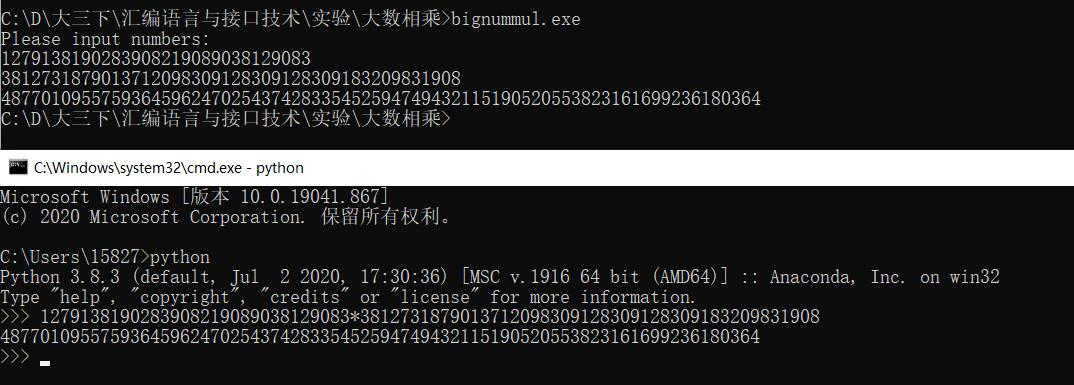
\includegraphics[width= 0.9\textwidth]{assets/大数乘法1}
    \caption{验证1}
    \label{验证1}
\end{figure}
\subsection{输入负数}
\begin{figure}[H]
    \centering
    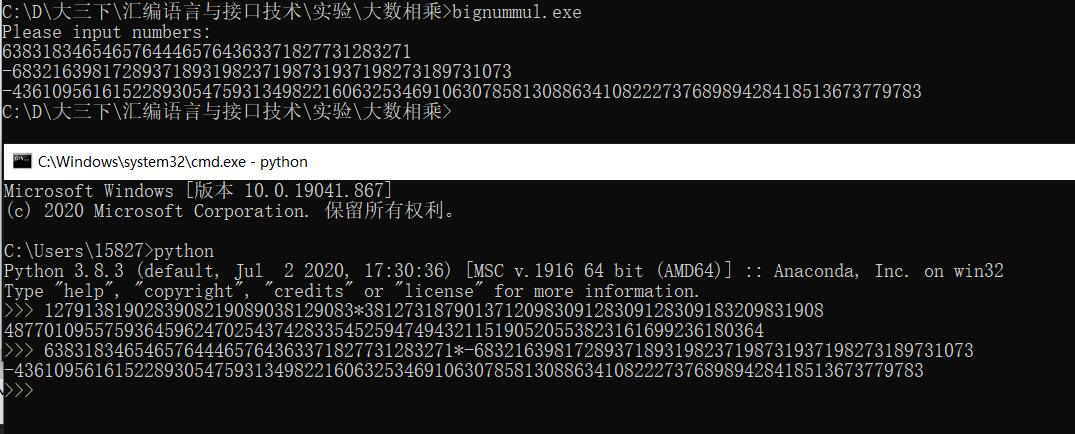
\includegraphics[width= 0.9\textwidth]{assets/大数乘法2}
    \caption{验证2}
    \label{验证2}
\end{figure}


\chapter{实验五——C语言多重循环反汇编分析}

\section{实验目的}
C语言编写多重循环程序(大于3重),查看其反汇编码,分析各条语句功能(分析情况需要写入实验报告),并采用汇编语言重写相同功能程序。

\section{实验步骤}
\begin{enumerate}
    \item 编写C语言四重循环的代码
    \item 在Visual Studio 2019中查看其反汇编代码并调试
    \item 分析反汇编代码各条语句的功能
    \item 采用MASM编写具有同样功能的代码
\end{enumerate}

\section{多重循环的C语言源码}
该程序作用为,从一个数组中选取四个数(可以相同),并计算这四个数
的和,输出这个数组中所有可能的和。

\begin{lstlisting}[language=C]
#include <stdio.h>

int a[10] = { 0, 1, 2, 3, 4, 5, 6, 7, 8 ,9 };

int main() {
    int n = 10;
    for (int i = 0; i < n; i++) {
        for (int j = 0; j < n; j++) {
            for (int k = 0; k < n; k++) {
                for (int m = 0; m < n; m++) {
                    int tmp = a[i] + a[j] + a[k] + a[m];
                    printf("%d\n", tmp);
                }
            }
        }
    }
}
\end{lstlisting}

\section{反汇编代码分析}
采用Visual Studio 2019自带的反汇编查看功能,对该程序生成的
反汇编码进行查看并分析各条语句的功能。

\subsection{初始化}

具体汇编码如下:
\begin{lstlisting}
005F4E90  push        ebp  
005F4E91  mov         ebp,esp  
005F4E93  sub         esp,108h  
005F4E99  push        ebx  
005F4E9A  push        esi  
005F4E9B  push        edi  
005F4E9C  lea         edi,[ebp-108h]  
005F4EA2  mov         ecx,42h  
005F4EA7  mov         eax,0CCCCCCCCh  
005F4EAC  rep stos    dword ptr es:[edi]  
005F4EAE  mov         ecx,offset _7E81AEF5_main@c (05FC003h)  
005F4EB3  call        @__CheckForDebuggerJustMyCode@4 (05F1208h)  
\end{lstlisting}

对上述汇编代码进行分析,进入main函数之后主要的初始化的流程如下:
\begin{enumerate}
    \item push        ebp: 保存调用者的栈指针
    \item mov         ebp,esp:使栈指针与帧指针的值相同
    \item sub         esp,108h:为当前函数开辟局部变量的空间, 这一步同上一步共同建立了一个新的栈帧
    \item line4~line6: 因为C语言函数中不允许修改这三个寄存器的值,因此把他们保存在堆中
    \item lea         edi,[ebp-108h]: 把栈帧的最低地址复制给edi
    \item line8~line10: 对栈帧中未初始化的数据进行初始化,其中ecx的值为DWORD的数量,eax的值为要储存的值,0CCCCCCCCh即代表未被初始化的值。rep指令的目的是重复其上面的指令,ECX的值是重复的次数.
\end{enumerate}

\subsection{定义局部变量并赋值}

具体汇编码如下:
\begin{lstlisting}
    ;int n = 10;
005F4EB8  mov         dword ptr [n],0Ah  
\end{lstlisting}

其中[n]代表着直接寻址。

\subsection{循环体}

按照编译原理中的基本块划分的思想,可以把这段代码做如下划分:
\begin{lstlisting}

    ;for (int i = 0; i < n; i++) {
005F4EBF  mov         dword ptr [ebp-14h],0     <——
005F4EC6  jmp         main+41h (05F4ED1h)  

\end{lstlisting}

\begin{lstlisting}

005F4EC8  mov         eax,dword ptr [ebp-14h]   <——
005F4ECB  add         eax,1  
005F4ECE  mov         dword ptr [ebp-14h],eax  

\end{lstlisting}

\begin{lstlisting}
    005F4ED1  mov         eax,dword ptr [ebp-14h]   <——
    005F4ED4  cmp         eax,dword ptr [n]  
    005F4ED7  jge         main+0E5h (05F4F75h)  
            ;for (int j = 0; j < n; j++) {
\end{lstlisting}

\begin{lstlisting}
    005F4EDD  mov         dword ptr [ebp-20h],0     <——
    005F4EE4  jmp         main+5Fh (05F4EEFh)  
\end{lstlisting}

\begin{lstlisting}
    005F4EE6  mov         eax,dword ptr [ebp-20h]   <——
    005F4EE9  add         eax,1  
    005F4EEC  mov         dword ptr [ebp-20h],eax 
\end{lstlisting}

\begin{lstlisting}
    005F4EEF  mov         eax,dword ptr [ebp-20h]   <——
    005F4EF2  cmp         eax,dword ptr [n]  
    005F4EF5  jge         main+0E0h (05F4F70h)  
                ;for (int k = 0; k < n; k++) {
\end{lstlisting}

\begin{lstlisting}
    005F4EF7  mov         dword ptr [ebp-2Ch],0     <——
                ;for (int k = 0; k < n; k++) {
    005F4EFE  jmp         main+79h (05F4F09h)  
\end{lstlisting}

\begin{lstlisting}
    005F4F00  mov         eax,dword ptr [ebp-2Ch]   <——
    005F4F03  add         eax,1  
    005F4F06  mov         dword ptr [ebp-2Ch],eax  
\end{lstlisting}

\begin{lstlisting}
    005F4F09  mov         eax,dword ptr [ebp-2Ch]   <——
    005F4F0C  cmp         eax,dword ptr [n]  
    005F4F0F  jge         main+0DBh (05F4F6Bh)  
                    ;for (int m = 0; m < n; m++) {
\end{lstlisting}

\begin{lstlisting}
    005F4F11  mov         dword ptr [ebp-38h],0     <——
    005F4F18  jmp         main+93h (05F4F23h)  
\end{lstlisting}


\begin{lstlisting}
    005F4F1A  mov         eax,dword ptr [ebp-38h]   <——
    005F4F1D  add         eax,1  
    005F4F20  mov         dword ptr [ebp-38h],eax  
\end{lstlisting}


\begin{lstlisting}
    005F4F23  mov         eax,dword ptr [ebp-38h]   <——
    005F4F26  cmp         eax,dword ptr [n]  
    005F4F29  jge         main+0D9h (05F4F69h)  
                        ;int tmp = a[i] + a[j] + a[k] + a[m];
\end{lstlisting}


\begin{lstlisting}
    005F4F2B  mov         eax,dword ptr [ebp-14h]   <——
                        ;int tmp = a[i] + a[j] + a[k] + a[m];
    005F4F2E  mov         ecx,dword ptr a (05FA000h)[eax*4]  
    005F4F35  mov         edx,dword ptr [ebp-20h]  
    005F4F38  add         ecx,dword ptr a (05FA000h)[edx*4]  
    005F4F3F  mov         eax,dword ptr [ebp-2Ch]  
    005F4F42  add         ecx,dword ptr a (05FA000h)[eax*4]  
    005F4F49  mov         edx,dword ptr [ebp-38h]  
    005F4F4C  add         ecx,dword ptr a (05FA000h)[edx*4]  
    005F4F53  mov         dword ptr [ebp-44h],ecx  
                        ;printf("%d\n", tmp);
    005F4F56  mov         eax,dword ptr [ebp-44h]  
    005F4F59  push        eax  
    005F4F5A  push        offset string "%d\n" (05F7BCCh)  
    005F4F5F  call        _printf (05F1375h)  
    005F4F64  add         esp,8  
                    ;}
    005F4F67  jmp         main+8Ah (05F4F1Ah)  
                ;}
\end{lstlisting}


\begin{lstlisting}
    005F4F69  jmp         main+70h (05F4F00h)     <——
            ;}
\end{lstlisting}


\begin{lstlisting}
    005F4F6B  jmp         main+56h (05F4EE6h)     <——
        ;}
\end{lstlisting}


\begin{lstlisting}
    005F4F70  jmp         main+38h (05F4EC8h)     <——
    ;}
\end{lstlisting}


\begin{lstlisting}
    005F4F75  xor         eax,eax                 <——
    005F4F77  pop         edi  
    005F4F78  pop         esi  
    005F4F79  pop         ebx  
    005F4F7A  add         esp,108h  
    005F4F80  cmp         ebp,esp  
    005F4F82  call        __RTC_CheckEsp (05F1212h)  
    005F4F87  mov         esp,ebp  
    005F4F89  pop         ebp  
    005F4F8A  ret
\end{lstlisting}

根据以上基本块的划分,可以画出程序的流程图如下:

\begin{figure}[H]
    \centering
    \includegraphics[width= 0.8\textwidth]{e:/CourseProject/Assembly/bigNumberMul/assets/tmp.pdf}
    \caption{循环体流程图}
    \label{循环体流程图}
\end{figure}

\section{采用MASM32重写该程序}

根据上述的程序流程图,在汇编中定义与其对应的代码块和跳转即可重写该
程序。与反汇编的代码的差别如下:
\begin{enumerate}
    \item 使用eax储存n,避免每次比较都需要执行mov eax, n
\end{enumerate}

部分关键代码如下:

\begin{lstlisting}
main proc    
    LOCAL i, j, k, m, tmp:DWORD
    mov eax, n

L0:
    mov i, 0
    jmp L2

L1:
    inc i

L2:
    cmp i, eax
    jge    L13    

L3:
    mov j, 0
    jmp L5

L4:
    inc j

L5:
    cmp j, eax
    jge L1

L6:
    mov k, 0
    jmp L8

L7:
    inc k

L8:
    cmp k, eax
    jge L4

L9:
    mov m, 0
    jmp L11

L10:
    inc m

L11:
    cmp m, eax
    jge    L7

L12:
    mov esi, i
    mov ecx, numbers[esi * 4]
    
    mov esi, j
    add ecx, numbers[esi * 4]

    mov esi, k
    add ecx, numbers[esi * 4]
    
    mov esi, m
    add ecx, numbers[esi * 4]

    mov tmp, ecx

    push eax
    invoke    printf, offset    string_d, tmp
    pop eax

    jmp L10

L13:
    ret    
main endp    
\end{lstlisting}

\section{实验结果展示}

由于四次循环会产生$n^4$个输出,因此本次测试让数组的长度为4,即
numbers = $\left\{1, 2, 3, 4\right\}$, 运行结果如下:

\begin{figure}[H]
    \centering
    \includegraphics[width= 0.9\textwidth]{e:/CourseProject/Assembly/bigNumberMul/assets/2020-06-05-15-11-24.png}
    \caption{多重循环实验结果-1}
    \label{多重循环实验结果-1}
\end{figure}

\begin{figure}[H]
    \centering
    \includegraphics[width= 0.9\textwidth]{e:/CourseProject/Assembly/bigNumberMul/assets/2020-06-05-15-12-04.png}
    \caption{多重循环实验结果-2}
    \label{多重循环实验结果-2}
\end{figure}

共64个输出,最小的为1+1+1+1=4,最大的为4+4+4+4=16,与C语言程序的
运行结果一致。

\chapter{多重循环分析}

\section{实验目的}
C语言编写多重循环程序(大于3重),查看其反汇编码,分析各条语句功能,并采用汇编语言重写相同功能程序。

\section{程序流程}
\begin{enumerate}
    \item 编写四重循环的C语言代码;
    \item 反汇编分析语句功能;
    \item 重写反汇编代码。
\end{enumerate}

\section{具体实现}
该节部分主要介绍了多重循环的C代码反汇编的分析以及代码的重写。
\subsection{多重循环的C语言代码}
设置四重循环,选取a数组中的四个数相加输出结果,其中为了方便显示不同循环次数,对每一次循环的边界值设定不一致。

具体代码如下:
\begin{lstlisting}
#include<stdio.h>
int a[10] = { 1,2,3,4,5,6,7,8,9 };
int main()
{
    for (int i = 0; i < 2; i++)
    {
        for (int j = 0; j < 3; j++)
        {
            for (int k = 0; k < 4; k++)
            {
                for (int m = 0; m < 5; m++)
                {
                    int sum = a[i] + a[j] + a[k] + a[m];
                    printf("%d\n", sum);
                }
            }
        }
    }
    return 0;
}
\end{lstlisting}

\subsection{反汇编分析}
点击调试后,查看反汇编得到汇编代码,并对语句进行分析。

分析过程如下:
\subsubsection{初始化}
\begin{lstlisting}
    00C61860  push        ebp  
    00C61861  mov         ebp,esp  
    00C61863  sub         esp,0FCh  
    00C61869  push        ebx  
    00C6186A  push        esi  
    00C6186B  push        edi  
    00C6186C  lea         edi,[ebp-0FCh]  
    00C61872  mov         ecx,3Fh  
    00C61877  mov         eax,0CCCCCCCCh  
    00C6187C  rep stos    dword ptr es:[edi]  
    00C6187E  mov         ecx,offset _B5E6F96D_多重循环@cpp (0C6C003h)  
    00C61883  call        @__CheckForDebuggerJustMyCode@4 (0C61316h) 
\end{lstlisting}
{\bfseries 1. push ebp}:将ebp压栈,保存调用函数的栈指针。
\\{\bfseries 2. mov ebp,esp}:把esp的值赋给ebp,也就是ebp指向栈基址
\\{\bfseries 3. sub esp,0FCh}:为当前函数开辟局部变量空间
\\{\bfseries 4. push ebx}
\\{\bfseries 5. push esi}
\\{\bfseries 6. push edi}:将ebx、esi、edi的值保存下来(压入栈中)
\\{\bfseries 7. lea edi,[ebp-0FCh]}:取出栈中局部变量区域(大小为0FCh=252的那一块)的最低地址
\\{\bfseries 8. mov ecx,3Fh}:把63赋给ecx
\\{\bfseries 9. mov eax,0CCCCCCCCh}:把0CCCCCCCCh赋给eax
\\{\bfseries 10. rep stos dword ptr es:[edi]}:将局部变量区域全部初始化为0CCCCCCCCh(这里63*4=252)

\subsubsection{内部循环体}
\begin{lstlisting}
	for (int i = 0; i < 2; i++)
;i=0
00C61888  mov         dword ptr [ebp-8],0  
00C6188F  jmp         main+3Ah (0C6189Ah)  
00C61891  mov         eax,dword ptr [ebp-8]  
00C61894  add         eax,1  
00C61897  mov         dword ptr [ebp-8],eax
;判断i是否<2  
00C6189A  cmp         dword ptr [ebp-8],2  
;如果不小于,跳出循环
00C6189E  jge         main+0D6h (0C61936h)  
	{
		for (int j = 0; j < 3; j++)
;j=0
00C618A4  mov         dword ptr [ebp-14h],0  
00C618AB  jmp         main+56h (0C618B6h)  
00C618AD  mov         eax,dword ptr [ebp-14h]  
00C618B0  add         eax,1  
00C618B3  mov         dword ptr [ebp-14h],eax 
;j<3? 
00C618B6  cmp         dword ptr [ebp-14h],3  
;跳到i的循环体里
00C618BA  jge         main+0D1h (0C61931h)  
		{
			for (int k = 0; k < 4; k++)
;k=0
00C618BC  mov         dword ptr [ebp-20h],0  
00C618C3  jmp         main+6Eh (0C618CEh)  
00C618C5  mov         eax,dword ptr [ebp-20h]  
00C618C8  add         eax,1  
00C618CB  mov         dword ptr [ebp-20h],eax  
;k<4?
00C618CE  cmp         dword ptr [ebp-20h],4  
跳到j的循环里
00C618D2  jge         main+0CCh (0C6192Ch)  
			{
				for (int m = 0; m < 5; m++)
00C618D4  mov         dword ptr [ebp-2Ch],0  
00C618DB  jmp         main+86h (0C618E6h)  
00C618DD  mov         eax,dword ptr [ebp-2Ch]  
00C618E0  add         eax,1  
00C618E3  mov         dword ptr [ebp-2Ch],eax  
00C618E6  cmp         dword ptr [ebp-2Ch],5 
;跳到k的循环里 
00C618EA  jge         main+0CAh (0C6192Ah)  
                    {
int sum = a[i] + a[j] + a[k] + a[m];
;取出a数组对应的值
00C618EC  mov         eax,dword ptr [ebp-8]  
00C618EF  mov         ecx,dword ptr a (0C6A000h)[eax*4]  
00C618F6  mov         edx,dword ptr [ebp-14h]  
00C618F9  add         ecx,dword ptr a (0C6A000h)[edx*4]  
00C61900  mov         eax,dword ptr [ebp-20h]  
00C61903  add         ecx,dword ptr a (0C6A000h)[eax*4]  
00C6190A  mov         edx,dword ptr [ebp-2Ch]  
00C6190D  add         ecx,dword ptr a (0C6A000h)[edx*4]  
00C61914  mov         dword ptr [ebp-38h],ecx  
					printf("%d\n", sum);
00C61917  mov         eax,dword ptr [ebp-38h]  
00C6191A  push        eax  
00C6191B  push        offset string "%d\n" (0C67B30h)  
00C61920  call        _printf (0C610CDh)  
;平衡堆栈
00C61925  add         esp,8  
				}
00C61928  jmp         main+7Dh (0C618DDh)  
			}
00C6192A  jmp         main+65h (0C618C5h)  
		}
00C6192C  jmp         main+4Dh (0C618ADh)  
	}
00C61931  jmp         main+31h (0C61891h)  
	return 0;
00C61936  xor         eax,eax  
}
\end{lstlisting}
根据上图展示的汇编代码以及相关注释,可以得到多重循环的逻辑结构。
\begin{figure}[H]
    \centering
    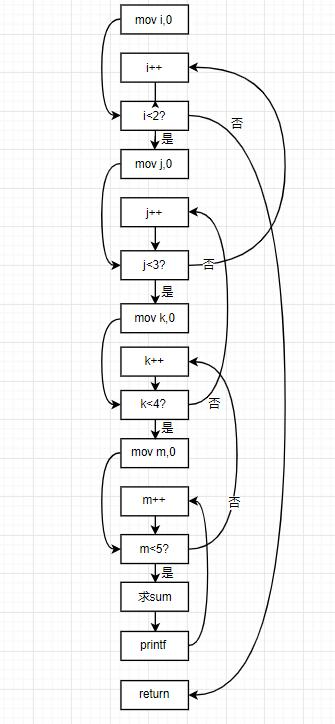
\includegraphics[width= 0.55\textwidth]{assets/多重循环}
    \caption{多重循环分析}
    \label{多重循环分析}
\end{figure}

\subsection{重写多重循环}
根据上述的代码逻辑结构,重写汇编程序如下:
\begin{lstlisting}
main proc
	local @i:dword,@j:dword,@k:dword,@m:dword,@sum:dword
	mov @i,0
	jmp L1
L4:
	add @i,1
L1:
	cmp @i,2
	jge L2
	mov @j,0
	jmp L3
L6:
	add @j,1
L3:
	cmp @j,3
	jge L4
	mov @k,0
	jmp L5
L8:
	add @k,1
L5:
	cmp @k,4
	jge L6
	mov @m,0
	jmp L7
L9:
	add @m,1
L7:
	cmp @m,5
	jge L8
	;计算sum
	mov eax,@i
	mov ecx,a[eax*4]
	mov eax,@j
	add ecx,a[eax*4]
	mov eax,@k
	add ecx,a[eax*4]
	mov eax,@m
	add ecx,a[eax*4]
	mov @sum,ecx
	;输出结果
	invoke printf,offset printStrlen,@sum
	jmp L9
L2:
	ret
	
main endp
end main
\end{lstlisting}
\section{实验结果展示}

% \subsection{两个文件相同}
\begin{figure}[H]
    \centering
    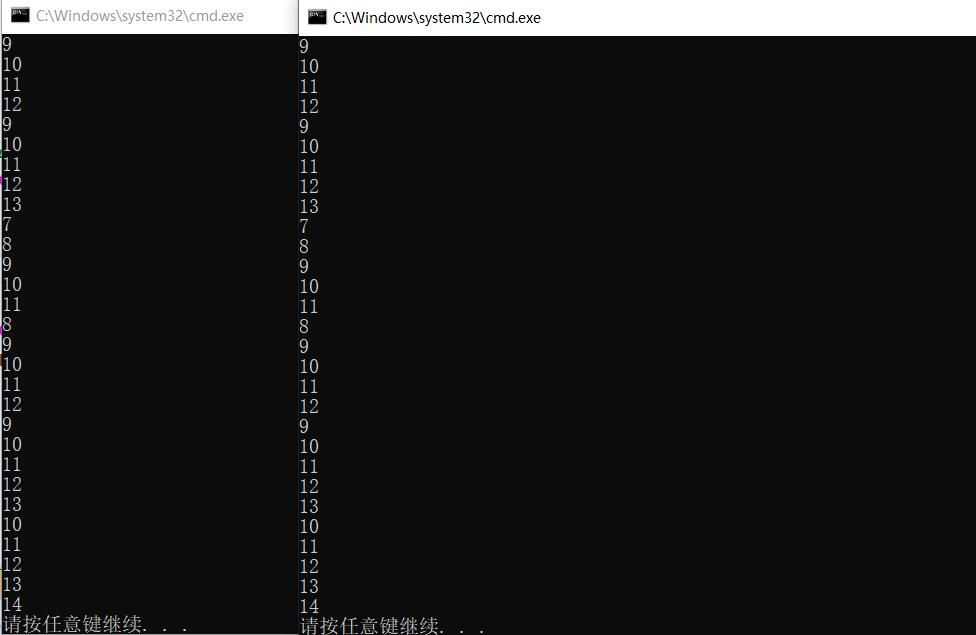
\includegraphics[width= 0.9\textwidth]{assets/多重循环结果}
    \caption{多重循环结果}
    \label{多重循环结果}
\end{figure}

% \subsection{两个文件内容不同}
% \begin{figure}[H]
%     \centering
%     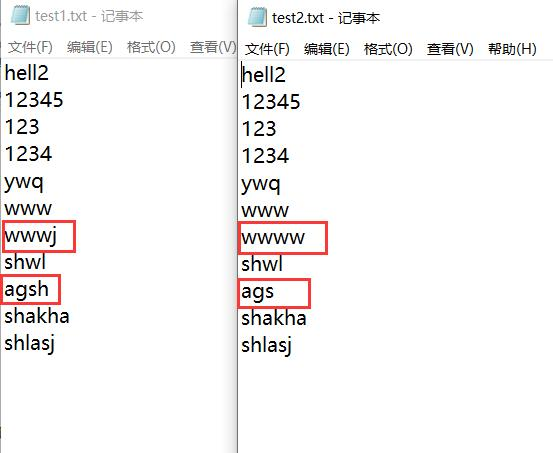
\includegraphics[width= 0.9\textwidth]{assets/文件比对2}
%     \caption{文件内容不同}
%     \label{文件内容不同}
% \end{figure}
% \begin{figure}[H]
%     \centering
%     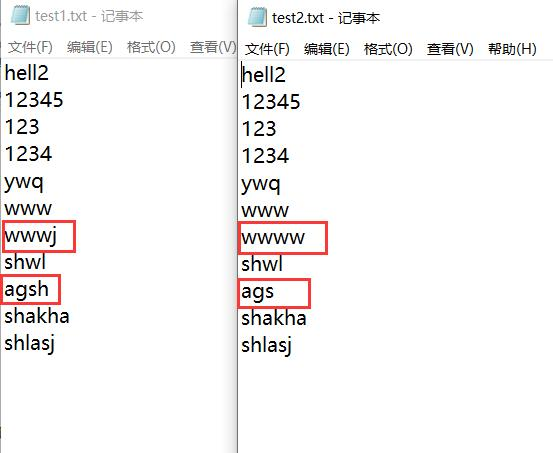
\includegraphics[width= 0.9\textwidth]{assets/文件比对2}
%     \caption{文件比对结果}
%     \label{文件比对结果2}
% \end{figure}


% % 结论:在结论相应的 TeX 文件处进行结论部分的撰写
%%
% The BIThesis Template for Bachelor Graduation Thesis
%
% 北京理工大学毕业设计(论文)结论 —— 使用 XeLaTeX 编译
%
% Copyright 2020 Spencer Woo
%
% This work may be distributed and/or modified under the
% conditions of the LaTeX Project Public License, either version 1.3
% of this license or (at your option) any later version.
% The latest version of this license is in
%   http://www.latex-project.org/lppl.txt
% and version 1.3 or later is part of all distributions of LaTeX
% version 2005/12/01 or later.
%
% This work has the LPPL maintenance status `maintained'.
%
% The Current Maintainer of this work is Spencer Woo.
%
% Compile with: xelatex -> biber -> xelatex -> xelatex

\unnumchapter{总~~~~结}
\renewcommand{\thechapter}{结论}

\ctexset{
  section/number = \arabic{section}
}

% 结论部分尽量不使用 \subsection 二级标题,只使用 \section 一级标题

% 这里插入一个参考文献,仅作参考
在该实验中,我采用MASM32和VS2019完成实验了大数相乘、文件比对和C语言多重循环分析这三个实验,总体上难度不大,我认为相比较麻烦一点的实验是文件比对,因为要用windows界面编程,我对里面的一些API不是很熟悉,
所以我采用了模块编程,先实现界面功能,再是文件比对,最后进行整合,这样一来,bug的数量就会减少一些。

这门课的实验偏向于底层,虽然和现在流行的编程语言有些脱离,但是靠近底层能帮助我们更好的理解计算机的运行机制,为程序的进一步优化也做好了铺垫。

感谢老师这一学期的辛苦讲授,我受益良多。

% \textcolor{blue}{结论作为毕业设计(论文)正文的最后部分单独排写,但不加章号。结论是对整个论文主要结果的总结。在结论中应明确指出本研究的创新点,对其应用前景和社会、经济价值等加以预测和评价,并指出今后进一步在本研究方向进行研究工作的展望与设想。结论部分的撰写应简明扼要,突出创新性。阅后删除此段。}

% \textcolor{blue}{结论正文样式与文章正文相同:宋体、小四;行距:22 磅;间距段前段后均为 0 行。阅后删除此段。}

% % 参考文献:如无特殊需要,参考文献相应的 TeX 文件无需改动,添加参考文献请使用 BibTeX 的格式
% %   添加至 misc/ref.bib 中,并在正文的相应位置使用 \cite{xxx} 的格式引用参考文献
% % %%
% The BIThesis Template for Bachelor Graduation Thesis
%
% 北京理工大学毕业设计(论文)参考文献 —— 使用 XeLaTeX 编译
%
% Copyright 2020 Spencer Woo
%
% This work may be distributed and/or modified under the
% conditions of the LaTeX Project Public License, either version 1.3
% of this license or (at your option) any later version.
% The latest version of this license is in
%   http://www.latex-project.org/lppl.txt
% and version 1.3 or later is part of all distributions of LaTeX
% version 2005/12/01 or later.
%
% This work has the LPPL maintenance status `maintained'.
%
% The Current Maintainer of this work is Spencer Woo.
%
% Compile with: xelatex -> biber -> xelatex -> xelatex
%
% 如无特殊需要,本页面无需更改

% 参考文献开始
\unnumchapter{参考文献}
\renewcommand{\thechapter}{参考文献}

% 设置参考文献字号为 5 号
\renewcommand*{\bibfont}{\zihao{5}}
% 设置参考文献各个项目之间的垂直距离为 0
\setlength{\bibitemsep}{0ex}
\setlength{\bibnamesep}{0ex}
\setlength{\bibinitsep}{0ex}
% 设置单倍行距
\renewcommand{\baselinestretch}{1.2}
% 设置参考文献顺序标签 `[1]` 与文献内容 `作者. 文献标题...` 的间距
\setlength{\biblabelsep}{0.5mm}
% 设置参考文献后文缩进为 0(与 Word 模板保持一致)
\renewcommand{\itemcmd}{
  \addvspace{\bibitemsep} % 恢复 \bibitemsep 的作用
  \mkgbnumlabel{\printfield{labelnumber}}
  \hspace{\biblabelsep}}
% 删除默认的「参考文献 / Reference」标题,使用上面定义的 section 标题

% -------------------------------- 示例内容 ------------------------------------- %
\textcolor{blue}{参考文献书写规范}

\textcolor{blue}{参考国家标准《信息与文献参考文献著录规则》【GB/T 7714—2015】,参考文献书写规范如下:}

\textcolor{blue}{\textbf{1. 文献类型和标识代码}}

\textcolor{blue}{普通图书:M}\qquad\textcolor{blue}{会议录:C}\qquad\textcolor{blue}{汇编:G}\qquad\textcolor{blue}{报纸:N}

\textcolor{blue}{期刊:J}\qquad\textcolor{blue}{学位论文:D}\qquad\textcolor{blue}{报告:R}\qquad\textcolor{blue}{标准:S}

\textcolor{blue}{专利:P}\qquad\textcolor{blue}{数据库:DB}\qquad\textcolor{blue}{计算机程序:CP}\qquad\textcolor{blue}{电子公告:EB}

\textcolor{blue}{档案:A}\qquad\textcolor{blue}{舆图:CM}\qquad\textcolor{blue}{数据集:DS}\qquad\textcolor{blue}{其他:Z}

\textcolor{blue}{\textbf{2. 不同类别文献书写规范要求}}

\textcolor{blue}{\textbf{期刊}}

\noindent\textcolor{blue}{[序号]主要责任者. 文献题名[J]. 刊名, 出版年份, 卷号(期号): 起止页码. }

\printbibliography [type=article,heading=none] 

\textcolor{blue}{\textbf{普通图书}}

\noindent\textcolor{blue}{[序号]主要责任者. 文献题名[M]. 出版地: 出版者, 出版年. 起止页码. }
\cite{Raymer1992Aircraft}

\printbibliography [keyword={book},heading=none] 

\textcolor{blue}{\textbf{会议论文集}}

\noindent\textcolor{blue}{[序号]析出责任者. 析出题名[A]. 见(英文用In): 主编. 论文集名[C]. (供选择项: 会议名, 会址, 开会年)出版地: 出版者, 出版年. 起止页码. }
\cite{sunpinyi}

\printbibliography [type=inproceedings,heading=none] 

\textcolor{blue}{\textbf{专著中析出的文献}}

\noindent\textcolor{blue}{[序号]析出责任者. 析出题名[A]. 见(英文用In): 专著责任者. 书名[M]. 出版地: 出版者, 出版年.起止页码. }
\cite{luoyun}

\printbibliography [type=inbook,heading=none] 

\textcolor{blue}{\textbf{学位论文}}

\noindent\textcolor{blue}{[序号]主要责任者. 文献题名[D]. 保存地: 保存单位, 年份. }
\cite{zhanghesheng}
\cite{Sobieski}

\printbibliography [keyword={thesis},heading=none] 

\textcolor{blue}{\textbf{报告}}

\noindent\textcolor{blue}{[序号]主要责任者. 文献题名[R]. 报告地: 报告会主办单位, 年份. }
\cite{fengxiqiao}
\cite{Sobieszczanski}

\printbibliography [keyword={techreport},heading=none] 

\textcolor{blue}{\textbf{专利文献}}

\noindent\textcolor{blue}{[序号]专利所有者. 专利题名[P]. 专利国别: 专利号, 发布日期. }
\cite{jiangxizhou}

\printbibliography [type=patent,heading=none] 

\textcolor{blue}{\textbf{国际、国家标准}}

\noindent\textcolor{blue}{[序号]标准代号. 标准名称[S]. 出版地: 出版者, 出版年. }
\cite{GB/T16159—1996}

\printbibliography [keyword={standard},heading=none] 

\textcolor{blue}{\textbf{报纸文章}}

\noindent\textcolor{blue}{[序号]主要责任者. 文献题名[N]. 报纸名, 出版年, 月(日): 版次. }
\cite{xiexide}

\printbibliography [keyword={newspaper},heading=none] 

\textcolor{blue}{\textbf{电子文献}}

\noindent\textcolor{blue}{[序号]主要责任者. 电子文献题名[文献类型/载体类型]. 电子文献的出版或可获得地址(电子文献地址用文字表述), 发表或更新日期/引用日期(任选). }
\cite{yaoboyuan}

\printbibliography [keyword={online},heading=none] 

\textcolor{blue}{关于参考文献的未尽事项可参考国家标准《信息与文献参考文献著录规则》(GB/T 7714—2015)}

% 在使用时,请删除/注释上方示例内容,并启用下方语句以输出所有的参考文献
% \printbibliography[heading=none]

% % 附录:在附录相应的 TeX 文件处进行附录部分的撰写
% % %%
% The BIThesis Template for Bachelor Graduation Thesis
%
% 北京理工大学毕业设计(论文)附录 —— 使用 XeLaTeX 编译
%
% Copyright 2020 Spencer Woo
%
% This work may be distributed and/or modified under the
% conditions of the LaTeX Project Public License, either version 1.3
% of this license or (at your option) any later version.
% The latest version of this license is in
%   http://www.latex-project.org/lppl.txt
% and version 1.3 or later is part of all distributions of LaTeX
% version 2005/12/01 or later.
%
% This work has the LPPL maintenance status `maintained'.
%
% The Current Maintainer of this work is Spencer Woo.
%
% Compile with: xelatex -> biber -> xelatex -> xelatex

\unnumchapter{附~~~~录}
\renewcommand{\thechapter}{附录}

% 设置附录编号格式
\ctexset{
  section/number = 附录\Alph{section}
}

附录相关内容…

% 这里示范一下添加多个附录的方法:

\section{\LaTeX 环境的安装}
\LaTeX 环境的安装。

\section{BIThesis 使用说明}
BIThesis 使用说明。

\textcolor{blue}{附录是毕业设计(论文)主体的补充项目,为了体现整篇文章的完整性,写入正文又可能有损于论文的条理性、逻辑性和精炼性,这些材料可以写入附录段,但对于每一篇文章并不是必须的。附录依次用大写正体英文字母 A、B、C……编序号,如附录 A、附录 B。阅后删除此段。}

\textcolor{blue}{附录正文样式与文章正文相同:宋体、小四;行距:22 磅;间距段前段后均为 0 行。阅后删除此段。}

% % 致谢:在致谢相应的 TeX 文件处进行致谢部分的撰写
% % %%
% The BIThesis Template for Bachelor Graduation Thesis
%
% 北京理工大学毕业设计(论文)致谢 —— 使用 XeLaTeX 编译
%
% Copyright 2020 Spencer Woo
%
% This work may be distributed and/or modified under the
% conditions of the LaTeX Project Public License, either version 1.3
% of this license or (at your option) any later version.
% The latest version of this license is in
%   http://www.latex-project.org/lppl.txt
% and version 1.3 or later is part of all distributions of LaTeX
% version 2005/12/01 or later.
%
% This work has the LPPL maintenance status `maintained'.
%
% The Current Maintainer of this work is Spencer Woo.
%
% Compile with: xelatex -> biber -> xelatex -> xelatex

\unnumchapter{致~~~~谢}
\renewcommand{\thechapter}{致谢}

\ctexset{
  section/number = \arabic{section}
}

% 致谢部分尽量不使用 \subsection 二级标题,只使用 \section 一级标题

值此论文完成之际,首先向我的导师……

\textcolor{blue}{致谢正文样式与文章正文相同:宋体、小四;行距:22 磅;间距段前段后均为 0 行。阅后删除此段。}


\end{document}
